\section{Апробация}

Решение было проверено и применено в рамках задачи отладки бортовой вычислительной системы мобильного робота [\ref{rokkit_bot}].

В рамках этой задачи требовалось получить данные об обменах на шине I2C между бортовым контроллером и EEPROM-памятью для хранения конфигурации мобильного робота. На шине регистрировалось большое количество обменов, так как работа с EEPROM в данной системе происходит в страничном режиме.

Ниже приведены представления данных в интерфейсе командной строки адаптера Bus Pirate и в среде Opermon.

\begin{lstlisting}[caption=Пример представления данных обменов в консольном интерфейсе Bus Pirate]
 [\\0xa0+\\0x00+\\0x00+[\\0xa1+\\0x00+\\0x00+\\0x00+\\0x00+\\0x00+\\0x00+\\0x00+\\0x00+\\0x00+\\0x00+\\0x00+\\0x00+\\0x00+\\0x00+\\0x00+\\0x00-][\\0xa0+\\0x00+\\0x10+[\\0xa1+\\0xa2+\\0x00+\\0xcc+\\0x00+\\0xac+\\0x00+\\0x00+\\0x00+\\0x00+\\0x00+\\0x00+\\0x00+\\0x00+\\0x00+\\0x00+\\0x00-][\\0xa0+...
\end{lstlisting}

\begin{figure}[H]
 \centering
 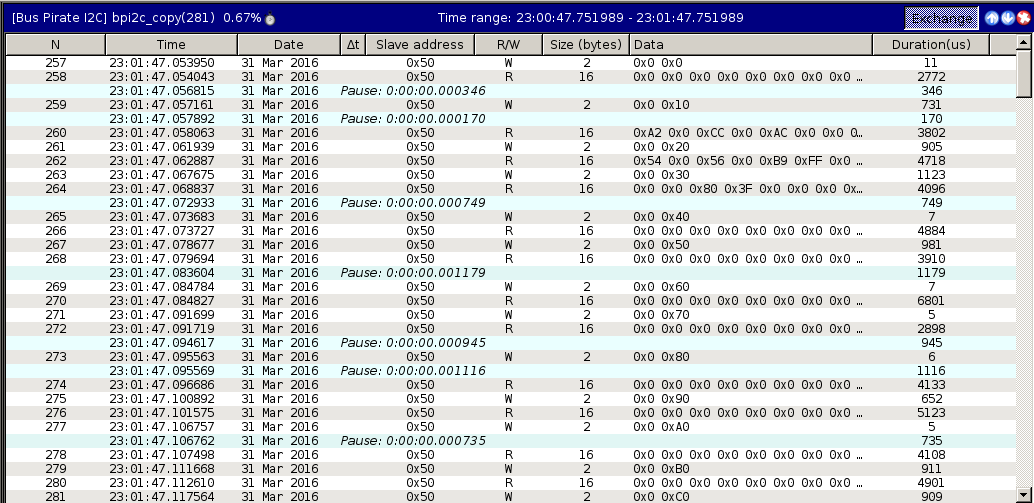
\includegraphics[width=\textwidth]{opermon-bp}
 \caption{Пример представления данных обменов в интерфейсе Opermon}
 \label{fig:opermon-bp}
\end{figure}

Очевидно, что работа с представлением данных в среде Opermon проще и информативней. Помимо содержимого обменов, которые, к тому же, оказываются разделёнными построчно, можно узнать длительность обмена и время его регистрации.